\documentclass{beamer}\usepackage[]{graphicx}\usepackage[]{color}
%% maxwidth is the original width if it is less than linewidth
%% otherwise use linewidth (to make sure the graphics do not exceed the margin)
\makeatletter
\def\maxwidth{ %
  \ifdim\Gin@nat@width>\linewidth
    \linewidth
  \else
    \Gin@nat@width
  \fi
}
\makeatother

\definecolor{fgcolor}{rgb}{0.345, 0.345, 0.345}
\newcommand{\hlnum}[1]{\textcolor[rgb]{0.686,0.059,0.569}{#1}}%
\newcommand{\hlstr}[1]{\textcolor[rgb]{0.192,0.494,0.8}{#1}}%
\newcommand{\hlcom}[1]{\textcolor[rgb]{0.678,0.584,0.686}{\textit{#1}}}%
\newcommand{\hlopt}[1]{\textcolor[rgb]{0,0,0}{#1}}%
\newcommand{\hlstd}[1]{\textcolor[rgb]{0.345,0.345,0.345}{#1}}%
\newcommand{\hlkwa}[1]{\textcolor[rgb]{0.161,0.373,0.58}{\textbf{#1}}}%
\newcommand{\hlkwb}[1]{\textcolor[rgb]{0.69,0.353,0.396}{#1}}%
\newcommand{\hlkwc}[1]{\textcolor[rgb]{0.333,0.667,0.333}{#1}}%
\newcommand{\hlkwd}[1]{\textcolor[rgb]{0.737,0.353,0.396}{\textbf{#1}}}%

\usepackage{framed}
\makeatletter
\newenvironment{kframe}{%
 \def\at@end@of@kframe{}%
 \ifinner\ifhmode%
  \def\at@end@of@kframe{\end{minipage}}%
  \begin{minipage}{\columnwidth}%
 \fi\fi%
 \def\FrameCommand##1{\hskip\@totalleftmargin \hskip-\fboxsep
 \colorbox{shadecolor}{##1}\hskip-\fboxsep
     % There is no \\@totalrightmargin, so:
     \hskip-\linewidth \hskip-\@totalleftmargin \hskip\columnwidth}%
 \MakeFramed {\advance\hsize-\width
   \@totalleftmargin\z@ \linewidth\hsize
   \@setminipage}}%
 {\par\unskip\endMakeFramed%
 \at@end@of@kframe}
\makeatother

\definecolor{shadecolor}{rgb}{.97, .97, .97}
\definecolor{messagecolor}{rgb}{0, 0, 0}
\definecolor{warningcolor}{rgb}{1, 0, 1}
\definecolor{errorcolor}{rgb}{1, 0, 0}
\newenvironment{knitrout}{}{} % an empty environment to be redefined in TeX

\usepackage{alltt}
\usetheme{Ilmenau}
\usepackage{amsmath,float,setspace,lmodern,graphicx,amsthm,amsfonts,multirow,hyperref,bm,bbm}

\setbeamertemplate{itemize items}[default]
\setbeamertemplate{enumerate items}[default]

\setbeamercovered{transparent}

\title[Reproducibility with \texttt{git} and \texttt{knitr}]{\texttt{GIT}ting started with reproducibility: \\ An introduction to \texttt{git} and \texttt{knitr}}
\author{Nick Seewald}
\subtitle{Biostatistics Student Association Computing Workshop}
\institute[University of Michigan]{Department of Statistics \\ University of Michigan}
\date{January 29, 2016}
% \logo{\includegraphics[height=.6cm]{blockm.png}}
\IfFileExists{upquote.sty}{\usepackage{upquote}}{}
\begin{document}
	
	\maketitle
	
	\section{Introduction}

	\begin{frame}{Why do I care about reproducibility?}
		Reproducible research is a hallmark of the scientific method, but we're pretty bad at it. 
		
		\begin{quote}
			In 2012, a researcher then at the biotechnology company Amgen wrote in Nature that when his team tried to reproduce 53 landmark cancer studies, they could replicate just six. And according to a news report in Nature, a project aiming to reproduce the findings of 100 psychology papers has managed to replicate results for only 39 of them (the project's findings are still under peer review).
		\end{quote}
		
		\footnotesize{''What Science Can Tell Us About Bad Science'', \textit{The Atlantic}, September 2015.} \scriptsize{\url{http://www.theatlantic.com/magazine/archive/2015/09/a-scientific-look-at-bad-science/399371/}}
	\end{frame}

	\begin{frame}{But I'm a Biostatistician!}
		\begin{itemize}
			\item Reproducibility is important in both science AND statistics!
			\item As statisticians, we need to be able to reproduce our results on the same data set
			\begin{itemize}
				\item This means we have to write reports in a way that minimizes error and write code so that we can get the same results years later.
			\end{itemize}
		\end{itemize}
	\end{frame}
	
	\begin{frame}{Agenda}
		\begin{enumerate}
			\item \texttt{Git}: A ``version control'' tool used for collaborating and maintaining different versions of a file, typically for code.
			\begin{itemize}
				\item Great for collaborating, or just saving your own ass.
				\item Often used in conjunction with \textit{GitHub}, an online repository storage service.
			\end{itemize}

			\item \texttt{knitr}: An R package that lets you create documents containing R code and output.
			\begin{itemize}
				\item Keep everything you need to generate a report (e.g., for research, homework, or 699) in one place!
				\item My favorite part: Update code without having to re-create tables! (This is where errors creep in!)
			\end{itemize}
		\end{enumerate}
	\end{frame}
	
	\section{\texttt{Git}}
	
	\begin{frame}{A brief warning}

  \begin{figure}
			\centering
			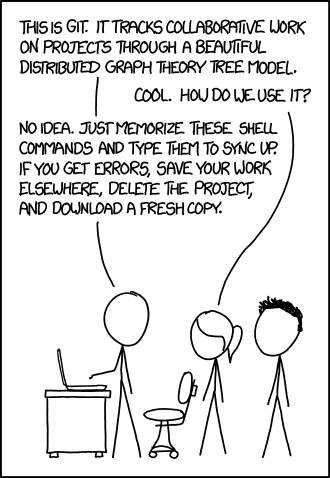
\includegraphics[height=.75\textheight]{xkcd-git.png}
		\end{figure}
		\scriptsize{Source: \url{https://xkcd.com/1597/}}
	\end{frame}
	
	\begin{frame}{Setup}
		Create a GitHub account, then download either Git or GitHub Desktop.
		\begin{itemize}
			\item Pure Git (i.e., just command-line tools): \url{https://git-scm.com/downloads}
			\item GitHub Desktop (GUI + command-line tools): \url{https://desktop.github.com/}
		\end{itemize}
	\end{frame}
	
	\section{\texttt{knitr}}
	
	\begin{frame}{What is \texttt{knitr}?}
		\begin{itemize}
			\item \texttt{knitr} lets you embed code and output from R into \LaTeX, HTML, RMarkdown, etc.
		\end{itemize}
	\end{frame}
	

\end{document}
